\documentclass[oneside,dutch]{tudelft-report}
\DeclareGraphicsExtensions{.pdf,.png,.jpg,.jpeg}
%\usepackage[numbered, framed]{mcode}
\usepackage{subcaption}
\usepackage{float}
\usepackage[dutch]{babel}
\usepackage{calc}  
\usepackage{enumitem}  
\usepackage{tabto}
\usepackage{adjustbox}
\usepackage{blindtext}
\usepackage{listings}
\usepackage{caption}



\title{Mid-term report}
\author{Projectgroep A2}
\affiliation{TU Delft}

\begin{document}
\maketitle

\tableofcontents
\mainmatter

\chapter{Inleiding}
EPO-3 is het derde project uit de propedeuse van de bachelor opleiding Electrical Engineeringaan de TU delft. Het doel van dit project is het ontwerpen van een chip, deze chip kan bijvoorbeeld een spelletje bevatten of als besturingsdoel dienen. Als project groep A5 is er gekozen voor het bouwen van een spelcomputer, hierop kunnen meerdere games gespeeld worden. De verschillende games moeten van een SD-kaart worden geladen voordat ze gespeeld kunnen worden. Het eerste spel dat ontworpen wordt is Pong, mocht er aan het eind van dit project nog tijd overblijven zullen er meerdere spellen volgen. De besturing loopt via ultrasone sensoren die de locatie van iemands hand bepalen. In dit tussentijdse ontwerp rapport zullen al deze onderdelen aanbod komen, daarbij moet vermeld worden dat ze nog niet geheel voltooid en getest zijn.  

\chapter{Probleemstelling}
\section{Projectopgave: 'Ontwerp een chip'}
De opdracht meegegeven door de TU is het ontwerpen van een chip. Hiermee is de gehele opdracht eigenlijk al beschreven, de studenten mogen verder in alle vrijheid de opdracht verder bepalen. Er wordt natuurlijk wel eerst grondig gecontroleerd door de tutoren of de opdrachten aan de eisen voldoen en haalbaar zijn.  Naast het ontwerpen van de chip mogen er extern onderdelen worden toegevoegd, bijvoorbeeld een beeldscherm of onderdelen voor de besturing. 

Als project groep A5 is er gekozen om van de chip een spelcomputer te maken, hierop moeten meerdere spellen gespeeld kunnen worden. Als eerst moet het spelletje 'Pong' te spelen zijn op deze spelcomputer. Aan het einde van het project kunnen eventueel andere spellen ontworpen worden. Extern moet er gezorgd worden voor besturing, weergave en opslag van de spellen. Dit laatste wordt door middel van een SD-kaart gerealiseerd. De besturing vind plaats via ultrasone sensoren of mocht dit niet naar behoren werken door middel van drukknoppen.

\section{Beschikbare infrastructuur}
In het 4e semester wordt de chip geproduceerd en getest, deze chip wordt door twee projectgroepen gebruikt. Elke groep heeft dus een halve chip voor zijn ontwerp, dit zijn ongeveer 200-250 flipflops. Daarnaast kan iedere groep wel gebruik maken van alle aansluitpinnen op de chip, dit zijn er 32. Voor het testen tussen door is er hardware beschikbaar, in de vorm van een Altera FPGA bord. Op dit Altera bord is veel randapparatuur aanwezig, daarnaast kunnen er nog andere externe onderdelen aan dit bord worden gekoppeld. 

\section{Functionele eisen}
Als functionele eisen kan er kortom gezegd worden dat er op de chip meerdere spellen gespeeld kunnen worden. Deze spellen moeten bestuurd kunnen worden door middel van ultrasone sensoren. Om te beginnen wordt 'Pong' ontworpen, andere spellen volgen als de projecttijd dit toelaat.

\section{Randvoorwaarden}
Aan het eindresultaat zitten een aantal randvoorwaarden verbonden. De externe onderdelen mogen maximaal 30 á 40 euro kosten, mochten deze niet voorhanden zijn. Er moet rekening worden gehouden met de grote van de chip. Tot slot dient aan alle tijdschema's te worden voldaan.

\section{Plan van aanpak}
Het plan van aanpak is een beschrijving van de aanpak van dit project, hierin staan onder andere de doelstellingen en wegen daar naar toe beschreven. Het plan van aanpak is te vinden in appendix A.

\chapter{Besturing}
Ons systeem wordt gespeeld doormiddel van 2 soorten besturing. De Ultrasone en de Button. De speler kan de modus selecteren doormiddel van een switch. Deze data van de buttons en de ultrasone worden verwerkt door een Arduino. Er is gekozen voor deze optie omdat de Arduino via SPI werkt. Hierdoor kan de SPI code getest worden en kunnen we het aantal pinnen dat gebruikt wordt laag houden. 

\section{Ultrasone}
Een unieke uitdaging van ons project is de Ultrasone besturing, de besturing werkt door middel van een (ultrasone)sensor aan de rechterzijde van de speler. Deze sensor meet met een speel ruimte van 75cm elke 11 milliseconde. Het aansturen van de ultrasone sensoren gaat doormiddel van een 2ms lange pulse op de IN-pin. Dit is de trigger van de SRF-04(de door ons gekozen ultrasone sensor). Hierna verzend de sensor zijn pulse, op dat moment wordt de OUT-pin ook hoog. Deze blijft hoog tot de gereflecteerde pulse weer binnen komt. Deze tijd wordt gedeeld door 2 omdat het geluid zowel de afstand heen als terug moet afleggen. Deze tijd wordt vervolgens geschaald naar afstand door hem door 29m/s(de snelheid van geluid in lucht) te delen. Hierna wordt de tijd teruggemapt(alles tussen de 0 en de 75 wordt terug geschaald naar 0 en 12). Deze waarde wordt voor player 2 4 bits geschoven naar links. En vervolgens wordt het signaal via de hierbovengenoemende SPI verstuurd naar de chip.

\section{Buttons}
Bij de buttons wordt een andere manier van werken gehanteerd, hier wordt de waarde van de plaatsvector onthouden(als integer). En naar gelang welke button geactiveerd wordt, wordt het signaal 1 verhoogd/verlaagd. Dit getal kan maximaal 12 bereiken en minimaal 0. Vervolgens wordt dit signaal voor player 2 ook verschoven, en daarna verzonden via SPI.

De getallen 0->12 voor player 1/2 zijn in gebruik, dit geeft ruimte om 13,14,15 te gebruiken voor andere doeleinde. 13 dient als getal om de Start van systeem aan te geven. 15 is de Reset van het systeem.
\newpage

\chapter{Blackbox}
\section{Functionele beschrijving}
Voor het genereren van de beelden worden twee SRAM chips gebruikt. De ene chip wordt uitgelezen door de VGA generator en er wordt naar de andere chip geschreven door de GPU. Als een frame geschreven is naar de SRAM chip wordt de chip waar net naar geschreven is verbonden met de VGA generator zodat deze uitgelezen kan worden. De chip die voorheen verbonden was met de VGA wordt doorverbonden met de GPU zodat daar vervolgens naar geschreven kan worden. Door deze techniek toe te passen blijft het beeld op het scherm stabiel. De BlackBox is de schakeling die dat mogelijk maakt.
\section{Inputs en outputs}
De SRAM chips, de VGA en de GPU communiceren met elkaar met behulp van SPI. De schakeling heeft dus twee SPI master aansluitingen voor VGA en de GPU en twee SPI slave aansluitingen voor de twee SRAM chips. Een SPI aansluiting bestaat uit vier signaallijnen. Dit zijn de serial clock (SCLK), master in slave out (MISO), master out slave in (MOSI) en slave select (SS). Ook heeft de schakeling nog een ingang om te selecteren welke SRAM chip verbonden is met de VGA generator en welke met de GPU.

\begin{figure}[H]
\center
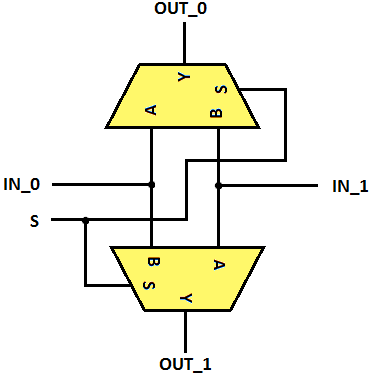
\includegraphics[width=9cm]{./BlackBox_Circuit}
\caption{Subschakeling van de blackbox}
\label{sub-blackbox}
\end{figure}

\section{Implementatie}
De schakeling bestaat uit vier subschakelingen. De subschakeling bestaat uit twee twee naar 1 lijn multiplexers zoals weergegeven in figuur 1. Door de S laag te maken, wordt IN\_0 verbonden met OUT\_0 en IN\_1 met OUT\_1. Als S hoog is, is IN\_0 verbonden met OUT\_1 en vice versa. Vervolgens worden de SCLK lijnen van de GPU en VGA generator verbonden met de ingangen van de subschakeling en de uitgangen met de SCLK lijnen van de twee SRAM chips. Hetzelfde gebeurt ook voor de MOSI en de SS lijnen van de masters en de slaves. Bij de MISO lijnen is het omgekeerd omdat dit een inputlijn is voor de masters en een outputlijn voor de slaves. Hier worden dus de SRAM chips verbonden met de ingangen en de VGA generator en de GPU aan de uitgangen. De BlackBox bestaat nu uit vier subcircuits. Door de select (S) ingangen van de subschakelingen met elkaar te verbinden is de BlackBox nu compleet.

\newpage

\chapter{CPU}
\section{Functionele beschrijving}
Om programma’s uit te kunnen voeren wordt gebruik gemaakt van een door de Delta-1 [INSERT BRON HIER] geïnspireerde microprocessor. Deze 8-bits processor krijgt instructies binnen die via SPI van een SD-kaart worden afgelezen. Vervolgens voert de processor bewerkingen uit, waarvan de resultaten doorgestuurd wordt naar de overige componenten op de chip. De data die uit de processor komt wordt hierna door de VGA-controller omgezet naar beelden op het scherm.

\begin{figure}[H]
\center
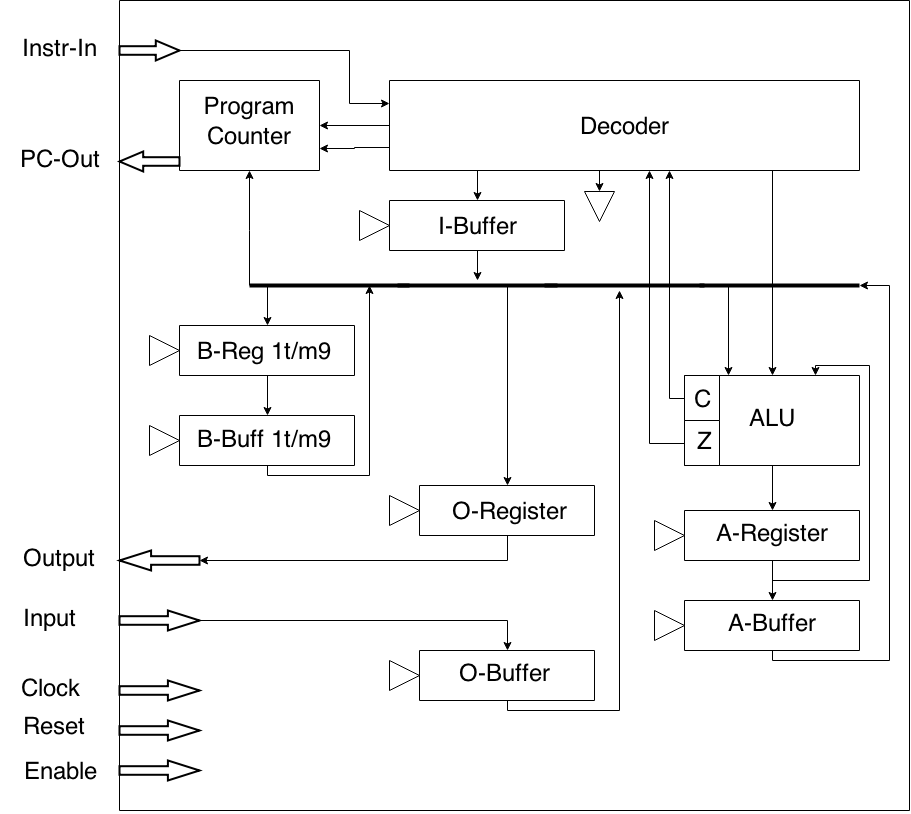
\includegraphics[width=9cm]{CPU-toplevel}
\caption{Toplevel beschrijving}
\label{CPU}
\end{figure}

\section{Inputs en outputs}
De processor heeft in totaal 5 ingangen. Dit zijn de 12-bits instructie-bus waarop de instructies staan die vanaf de SD kaart worden afgelezen, een 8-bits signaal waar alle externe inputs op komen te staan, de klok, de reset en het CPU-enable signaal. Het CPU-enable signaal geeft door aan de processor dat een nieuwe instructie klaar staat om uitgevoerd te worden. Op het 8-bits signaal waar alle inputsinformatie op staat, staat bijvoorbeeld de positie van de aansturing.
Verder beschikt de CPU over 2 uitgangen: Eén 8-bits signaal dat data naar de VGA controller stuurt en een 8-bits signaal dat het adres van de volgende instructie doorgeeft aan de SD-kaart uitlezer. 

\section{Implementatie}
De totale processor is opgebouwd uit 5 verschillende sub-schakelingen: Registers, buffers, een rekenkern, een program-counter en een instructie-decoder.

De processor beschikt in totaal over 11 registers. Wanneer het enable-signaal vanaf de decoder van een register hoog is, slaat deze de waarde die op dat moment aan zijn ingang staat op en kan deze data bij een later bewerking weer uitgelezen worden. Hiervan worden er 9 gebruikt om waarden op te slaan voor volgende bewerkingen, één om data aan de data-uitgang van de processor te zetten en één aan de uitgang van de rekenkern om direct een volgende bewerking op uit te kunnen voeren.

Verder zijn er 13 buffers aanwezig. Deze buffers laten data van hun ingang door naar hun uitgang wanneer hun enable-signaal vanaf de decoder hoog is, en geven 'high-Z' door wanneer dit niet zo is. Negen van deze 8-bits buffers staan tussen de uitgangen van de opslag-registers en de databus, één aan de controller-input, één tussen het rekenkern-register en de databus, één die vanuit de decoder een numerieke waarde op de databus kan zetten en één 12-bits buffer aan de instructie-ingang van de CPU.

De rekenkern heeft één 3-bits instructie-ingang vanuit de decoder, twee 8-bits data ingangen waarvan er een van de databus komt en een het resultaat van de vorige bewerking bevat, een 1-bit carry uitgang die aangeeft wanneer er een overflow optreedt bij een optel-operatie, een 1-bit zero uitgang die aangeeft wanneer een 'AND' operatie enkel nullen oplevert en een 8-bits uitgang waar het resultaat van de bewerkingen op staat. Afhankelijk van het instructie-signaal wordt een andere operatie uitgevoerd met de data op de twee ingangen. 

De program counter krijgt na elke instructie van de decoder een signaal om ofwel één instructie verder te gaan, of om naar een specifieke instructie te 'springen'. Dit wordt gedaan met behulp van een 1-bit increment en -jump signaal. Zolang de increment ingang hoog is wordt er telkens één opgeteld bij iedere instructie, en als het jump signaal hoog is wordt het nieuwe instructie-nummer vanaf de databus uitgelezen. Het 8-bits uitgangssignaal bevat het adres van de volgende instructie en wordt doorgegeven naar de SD-kaart uitlezer.

Aan de kern van de processor bevindt zich de instructie decoder. Deze decoder stuurt naar aanleiding van een 12-bits instructie de overige componenten binnen de CPU aan. Dit wordt gedaan door eerst het 12-bits signaal op te delen in een 4-bits instructie en een 8-bits argument. Hierna wordt afhankelijk van de instructie een enable-signaal naar een relevant register of buffer, een instructie-code naar de rekenkern en een increment of jump signaal naar de program counter gestuurd. Het 8-bits argument kan ofwel als waarde op de databus gezet worden of als enable-signaal omgezet worden voor een register of buffer. De mogelijke instructies met bijbehorende uitgangssignalen van de decoder zijn te zien in tabel [figuur 6.2]


\begin{figure}[H]
\center
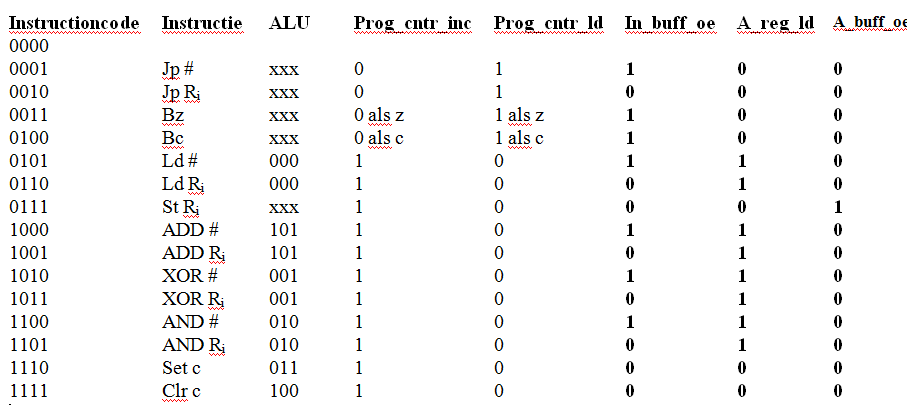
\includegraphics[width=9cm]{tabel}
\caption{Instructies met bijbehorende uitgangssignalen}
\label{CPU}
\end{figure}


\chapter{GPU}
De GPU is een component dat via de outputbuffer van de CPU 2 8 bit commando’s zal ontvangen met daarom achtereenvolgens de X en Y positie van de in te kleuren pixel op het scherm. Tevens zal er een commando bestaan om het volledige scherm schoon te vegen (Alle pixels uitzetten). De GPU ontvangt deze coördinaten en rekent dit om naar het adres waar de waarde ‘1’ of ‘0’ ingevuld zal moeten worden in het SRAM. Tevens bevind zich in de GPU de aansturing van het SRAM, via SPI. Deze zal bestaan uit een 8 bits instructiecode voor de schrijf handeling, gevolgd door een 16 bits adres waar de waarde geschreven zal moeten worden en uiteindelijk de waarde zelf. Op deze manier kan het SRAM geschreven worden vanuit de CPU en is het mogelijk om beeld te genereren.

De GPU is ontworpen aan de hand van een FSM, deze bevat 5 states en staat hieronder weergegeven.

\begin{figure}[H]
\center
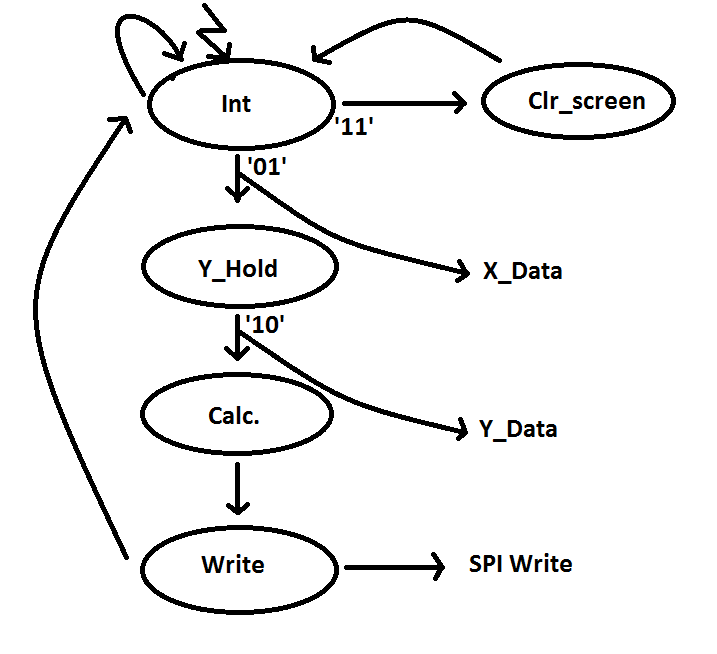
\includegraphics[width=9cm]{FSM_GPU}
\caption{Final State Machine van de GPU}
\label{sub-GPU}
\end{figure}

In de eerste state kan de GPU drie richtingen op gaan. Als de eerste twee bits van de 8-bits vector '11' zijn gaat de GPU naar Clr-screen,hier zal de VGA zijn scherm leeg maken. De GPU gaat zijn X-data inlezen en springt naar de volgende state (Y-Hold) als de eerste twee bits van de 8-bits vector '01' is. Voor iedere andere waarde op de eerste twee bits van de 8-bits vector blijft de GPU in de int state. Vanuit de Clr-screen state kan de GPU alleen nog maar terug naar de int state en begint de FSM opnieuw. In de Y-Hold state wacht de GPU op Y-Data, de GPU blijft in deze state totdat de eerste twee bits van de 8-bits vector '10' aangeven (Duurt 20 klokslagen). Op dat moment leest de GPU de Y-Data in en stapt over naar de Calc. state. In deze state wordt het adres berekend voor de VGA, dit gebeurd met de formule $32*Y+X =$ adres. Als deze berekening voor het bepalen van zijn adres is voltooid springt de GPU automatisch naar de volgende state, de Write state. In de Write state schrijft de GPU data uit de buffers weg via SPI. Automatisch zal de GPU terug springen naar zijn eerste state, het proces begint dan opnieuw. 

\chapter{VGA}
Functionele beschrijving
Om een monitor met een VGA aansluiting aan te sturen, zijn er eigenlijk 5 pinnen nodig die aangestuurd moeten worden. Drie pinnen voor rood, groen en blauw, een voor H-Sync en een voor V-Sync. 

\begin{figure}[H]
\center
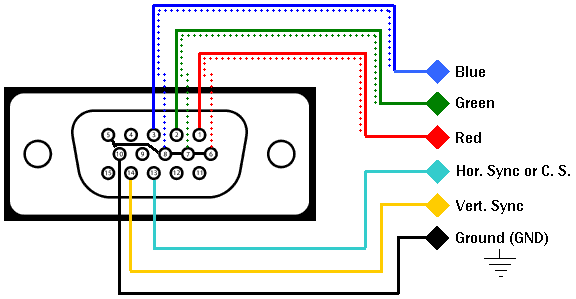
\includegraphics[width=9cm]{VGA-1}
\caption{Layout VGA-stekker}
\label{VGA}
\end{figure}

Dit is de layout van de een VGA-stekker. 

\section{RGB}
Op de pinnen voor rood, groen en blauw, staat een analoog signaal tussen de 0 en de 0.7 volt. Hoe hoger de spanning, hoe feller de kleur. Door middel van verschillende spanningsniveaus kan de kleur per pixel worden bepaald. Wij maken echter alleen gebruik van zwart en wit. Daarom wordt er slechts een signaal naar de alle RGB pinnen verstuurd. Hierdoor ontstaat een witte pixel. Wanneer dit niet gebeurt, is de pixel zwart. 

\section{H-Sync}
H-Sync vertelt de monitor wanneer een regel klaar. Als H-Sync laag is, betekent dit voor de monitor dat er een nieuwe regel pixels geschreven kan worden. Het is echter niet zo dat wanneer H-Sync weer hoog is, dat er gelijk pixels geschreven kunnen worden. Er zit nogal enige vertragingstijd ingebouwd. Deze tijd was bij CRT-monitoren nodig om elektronenstraal terug naar het begin te richten.

\begin{figure}[H]
\center
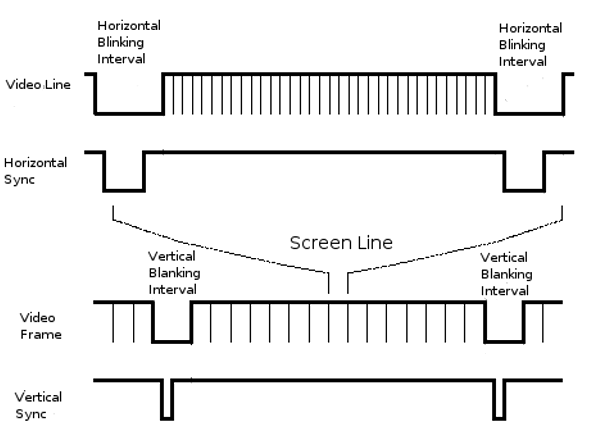
\includegraphics[width=9cm]{VGA-2}
\caption{}
\label{VGA}
\end{figure}

Video Line is het RGB signaal. Zoals te zien is in figuur 8.2, zit er tijd voor en na de dip van de H-sync. Deze tijd heet de front-porch en de back-porch. 

\section{V-Sync}
V-Sync is het signaal dat aan de monitor vertelt dat een volledig scherm is volgeschreven. Als V-Sync laag wordt, begint het scherm weer links bovenin met pixels vullen. Net als bij de H-Sync is er sprake van een Front-porch en een back-porch. Deze zijn bij de V-Sync een stuk langer dan bij de H-sync. Dit komt omdat de monitor de elektronenstraal van rechts onderin naar links bovenin moet sturen. Deze afstand is een stuk groter dan terug van rechts naar links. 

\section{Implementatie}
De VGA zet een serieel signaal om in een signaal dat voor een monitor te begrijpen is. Hiervoor zijn H-Sync, V-Sync en Von nodig. Von is eigenlijk hetzelfde signaal als H-sync. Het verschil is echter dat bij V-on de frontporch en de backporch zijn meegerekend. Von geeft aan de blackbox aan dat er een serieel signaal geschreven mag worden per 5 klokslagen.  Iedere vijf klokslagen wordt er een nieuwe pixel geschreven (eigenlijk zijn dat 20 pixels op het scherm). 

H-Sync wordt bepaald door een kloksignaal te tellen. Vervolgens wordt op basis van H-Sync de V-Sync bepaald. Dit gebeurd door te tellen hoe vaak H-Sync naar nul gaat. 

\chapter{SPI}
Serial Peripheral Interface in het kort ook SPI genoemd is een de facto-standaard die ooit door Motorola bedacht is voor het communiceren met randapparatuur, zoals embedded systems, sensors en memory cards. Bij SPI heb je de master en de slave deze communiceren met elkaar via twee seriële datalijnen daarnaast is er nog een kloklijn die aangeeft wanneer er data overgedragen wordt. De kloklijn wordt aangestuurd door de master, dit houdt in dat de slave niet kan pauzeren en altijd data aan de master aan moet bieden. De standaard definieert enkel hoe de data van de master naar de slave en vice versa over wordt gedragen, niet hoe de data verwerkt wordt, dit heeft als gevolgd dat randapparatuur zelf nog moet definiëren hoe de communicatie verloopt.

\section{Functionele beschrijving}
De SPI module begint met zenden/ontvangen zodra het send signaal hoog is en stopt zodra er acht bits zijn verzonden/ontvangen, daarna kunnen de ontvangen bits uitgelezen worden en nieuwe bits in worden geladen om te verzenden. Het overbrengen van het shift register dat in de master zit naar de slave en vice versa deze shift registers zijn in een kring op elkaar aangesloten, waarbij altijd de meest significante bit wordt verzonden. Voor de communicatie met de slave wordt een slave klok signaal gegenereerd, de data overdracht is gesynchroniseerd ten opzicht van dit signaal. Data wordt gesampled op de opgaande klokflank en de data wordt geshift op de neergaande klokflank.

\section{Inputs en outputs}
Hieronder een beschrijving van alle in- en outputs van de SPI module zoals te zien in figuur \ref{spi-diagram}.
\begin{itemize}
\item Clock: het kloksignaal waarop de SPI draait, het slave clock signaal zal dezelfde frequency hebben als dit kloksignaal
\item Reset: de hoofd reset van de SPI
\item Send: de input die aangeeft wanneer er begonnen moet worden met zenden/ontvangen
\item Write\_enable: als deze hoog is zal write\_in(8) in het shift register geladen worden
\item Write\_in(8): de bits die naar het shift register worden geschreven als write\_enable hoog is
\item Read\_out(8): de waarde die in het shift register staat
\item Slave clock: het slave kloksignaal die de communicatie met de slave aanstuurt
\item MOSI: de datalijn van de master naar de slave
\item MISO: de datalijn van de slave naar de master
\end{itemize}

\begin{figure}[H]
\center
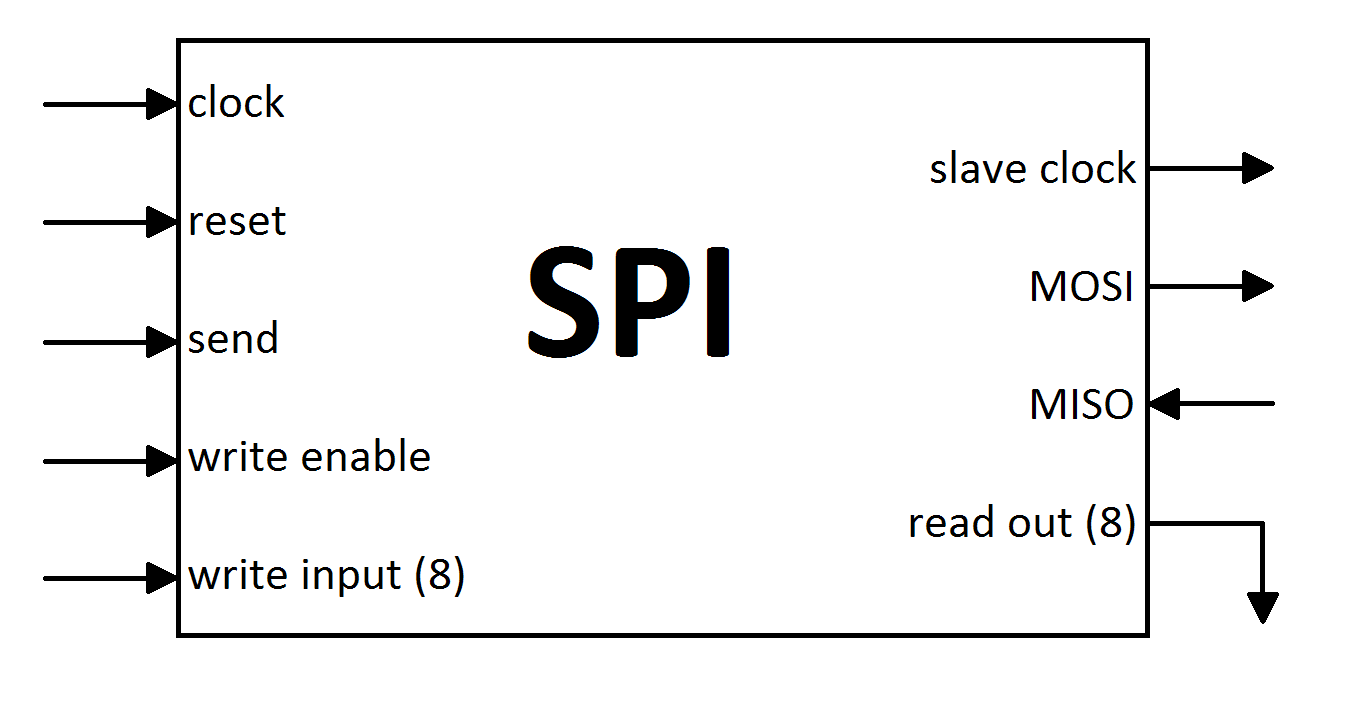
\includegraphics[width=9cm]{./spi_diagram}
\caption{Diagram of SPI circuit}
\label{spi-diagram}
\end{figure}

\section{Implementatie}
Voor de implementatie van de SPI is er voor gekozen om het in drie subsystemen op te delen:
\begin{itemize}
\item Counter: een simpele teller die de opgaande klokslagen van het slave clock signaal telt. 
\item Shift register: een shift register van acht bits die shift op de neergaande klokflank als het enable signaal hoog is en nieuwe waardes inlaad als de write enable hoog is. Het blokschema van het shift register is te zien in figuur \ref{shift-register-diagram}.
\item Control: een statemachine die er voor zorgt dat de SPI stopt met shiften na 8 klokslagen van de slave klok, zodat er tijd is om het register uit te lezen of nieuwe waarden in te laden. Het blokschema van Control is te zien in figuur \ref{control-diagram}.
\end{itemize}

Deze drie subsystemen zijn aan elkaar verbonden volgens het schema in figuur \ref{spi-system-diagram}.

\begin{figure}[H]
\centering
\begin{minipage}{.5\textwidth}
  \centering
  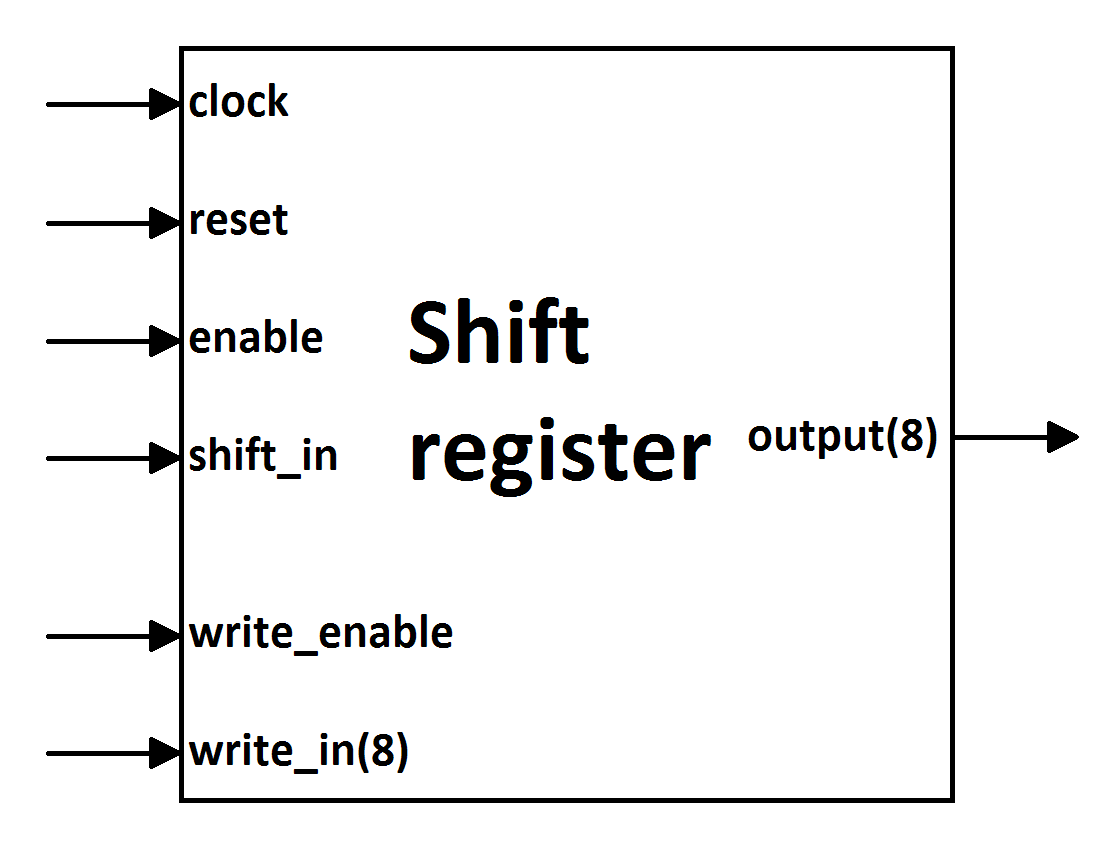
\includegraphics[width=5.4cm]{./shift_register_diagram}
  \captionof{figure}{Diagram van Shift regiser}
  \label{shift-register-diagram}
\end{minipage}%
\begin{minipage}{.5\textwidth}
  \centering
  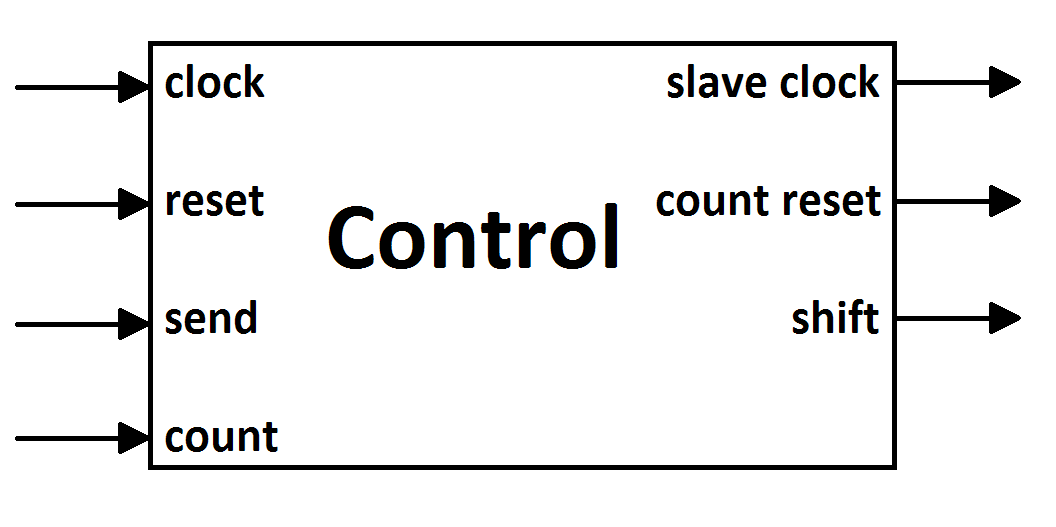
\includegraphics[width=7.8cm]{./control_diagram}
  \captionof{figure}{Diagram van Control} 
  \label{control-diagram}
\end{minipage}
\end{figure}

\begin{figure}[H]
\center
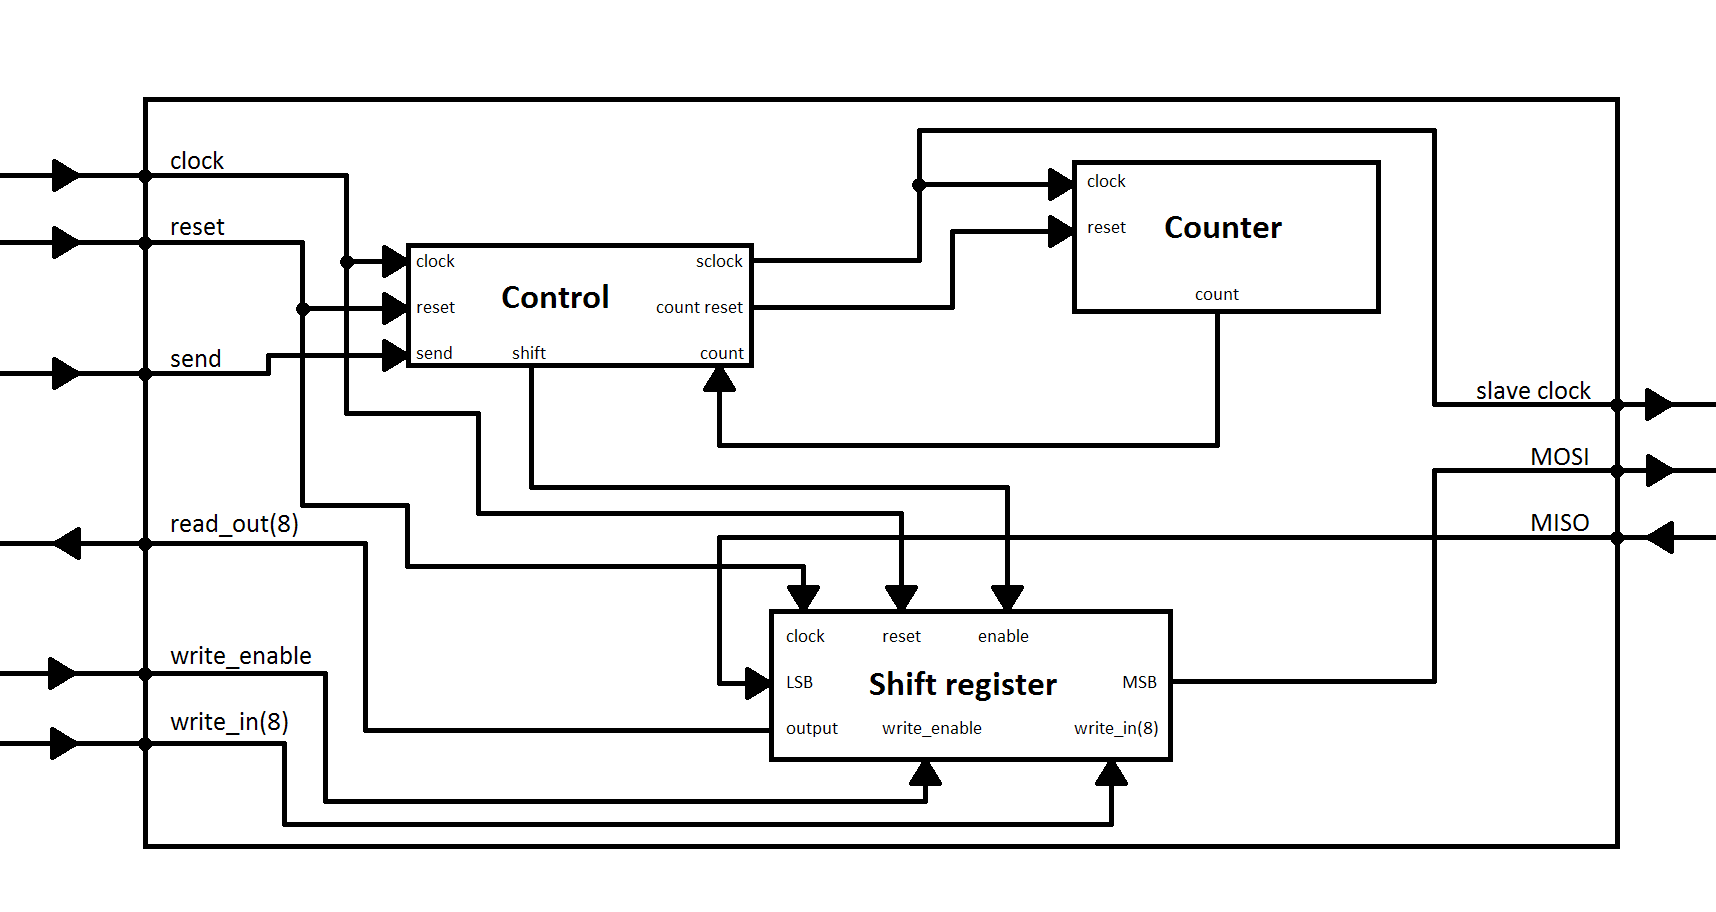
\includegraphics[width=11.4cm]{./spi_system_diagram}
\caption{Diagram van de verbinding van de componenten}
\label{spi-system-diagram}
\end{figure}

\newpage

\chapter{SD-kaart}
Voor het opslaan van de instructies voor de CPU is gekozen voor een SD-kaart. Voor het uitlezen van een SD-kaart zijn er drie verschillende modes, twee hiervan zijn echter gebaseerd op een zelf ontworpen systeem van SanDisk. De derde mode is echter gebaseerd op SPI waarvan al een module is die al ontworpen is, daarom is hier ook voor gekozen. 
\section{SD communicatie}
Aangezien SPI niets zegt over hoe de communicatie verloopt of wat de betekenis van de overgebrachte data is, definieert SanDisk in de SD specificatie een aantal commando’s die naar de SD-kaart gestuurd kunnen worden. Er zal niet specifiek in worden gegaan op wat deze commando’s zijn, je moet denken aan: reset, lezen en schrijven commando’s, er zal wel ingegaan worden op hoe deze commando’s worden gestuurd en wat de reacties hier op zijn.
\section{SD commando's \& responses}
De communicatie met de SD-kaart verloopt als volgt: er wordt een commando naar de SD-kaart verstuurt, de SD-kaart geeft antwoordt of het een correct commando is en of het commando verwerkt kan worden, daarna komt eventueel nog, bij het lezen, data van de SD-kaart of, bij het schrijven, data naar de SD-kaart. Zodra alles is afgehandeld kan er een nieuw commando gestuurd worden.
\section{Functionele omschrijving}
De SD module is zo ontworpen dat deze een adres binnen krijgt van de program counter van de CPU deze uitleest vanaf de SD-kaart en deze vervolgens aanbiedt aan de CPU. Zolang de SD module nog bezig is met het uitlezen van het adres zal het busy signaal hoog zijn.

\begin{figure}[H]
\center
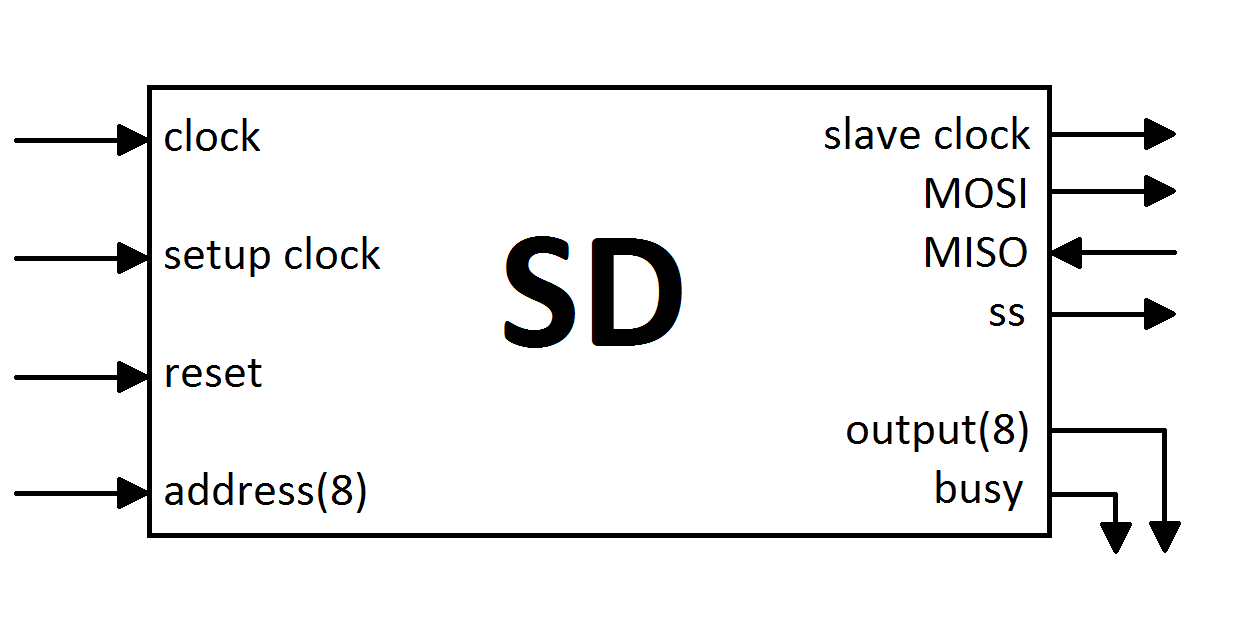
\includegraphics[width=9cm]{./sd_diagram}
\caption{Diagram of SD circuit}
\label{sd-diagram}
\end{figure}

\newpage

\section{Inputs en outputs}
Hieronder een beschrijving van alle in- en outputs van de SD module zoals te zien in figuur \ref{sd-diagram}.

\begin{itemize}
\item Clock: het kloksignaal waar de SD module op draait, dit is ook het kloksignaal waar de SPI na initialisatie op zal draaien
\item Setup clock: het kloksignaal dat tijdens de initialisatie gebruikt zal worden, deze moet tussen de 100 en 400 kHz liggen
\item Reset: het algemene reset signaal 
\item Address: het adres dat van de SD-kaart zal worden afgelezen
\item Output(8): dit zal de waarde zijn die op het adres staat zodra deze is uitgelezen
\item Busy: dit signaal geeft aan of de SD module bezig is
\item Slave clock: het slave kloksignaal dat de SD-kaart aanstuurd
\item MOSI: de datalijn van de SD module naar de SD-kaart
\item MISO: de datalijn van de SD-kaart naar de SD module
\item SS: het slave select signaal, dit signaal wordt gebruikt om de SD-kaart in SPI mode te krijgen en om aan te geven dat de SD-kaart geselecteerd is.
\end{itemize}


\chapter{Discussie}
Over het eindontwerp is nog geen discussie mogelijk. Voor het schrijven van dit tussentijdse ontwerprapport zijn er nog wel een aantal dingen naar voren gekomen. Voorop staat het feit dat alles minder snel en soepel verloopt als dat we gehoopt hadden. Het testen van de hardware op het FPGA bord bracht veel oponthoud met zich mee. Ook bleken de stappen die tot het eindproduct moesten lijden niet compleet bedacht, tijdens het ontwerpproces kwamen er extra stappen naar voren die veel tijd hebben gekost. Ondanks dat de einddatum steeds dichterbij komt denken we dat alles binnen de tijd realiseerbaar is.

\end{document}